\begin{pregunta}
\puntaje{5}
\begin{cuerpo}
Dos tanques inicialmente llenos de $20[L]$ de un reactivo se conectan mediante dos bombas, una transporta a un caudal constante de $0.05[L/s]$ y la otra a $0.65[L/s]$. 
\begin{center}
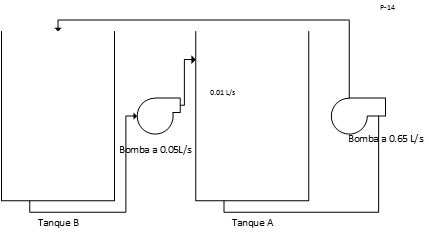
\includegraphics[width=0.8\textwidth]{./img/p19.jpg}
\end{center}
¿C\'ual de los siguientes ruteros permite encontrar el volumen contenidos en ambos tanques en funci\'on del tiempo?.
\end{cuerpo}

\begin{multicols}{2}
\begin{alternativas}
{
\texttt{f=@(t,v) [0.65-0.05;0.05-0.65];}\\
\texttt{[t,v]=ode45(f,[0,35],[20;20]);}\\
\texttt{plot(t,v)} }
{
\texttt{f=@(t,v) [0.65;0.05];}\\
\texttt{[t,v]=ode45(f,[0,35],[20;20]);}\\
\texttt{plot(t,v)} }
{
\texttt{f=@(t,v) [0.05;-0.65];}\\
\texttt{[t,v]=ode45(f,[0,35],[20;20]);}\\
\texttt{plot(t,v)} }
{
\texttt{f=@(t,v) [0.65-0.05;0.05-0.65];}\\
\texttt{[t,v]=ode45(f,[0,35]);}\\
\texttt{plot(t,v)} }
\end{alternativas}
\end{multicols}
\justificacion{8cm}
\end{pregunta}